\documentclass[class=article, crop=false]{standalone}
\usepackage{tikz}
\usepackage{subcaption}
\usetikzlibrary{calc}
\usetikzlibrary {shapes.geometric}

\begin{document}
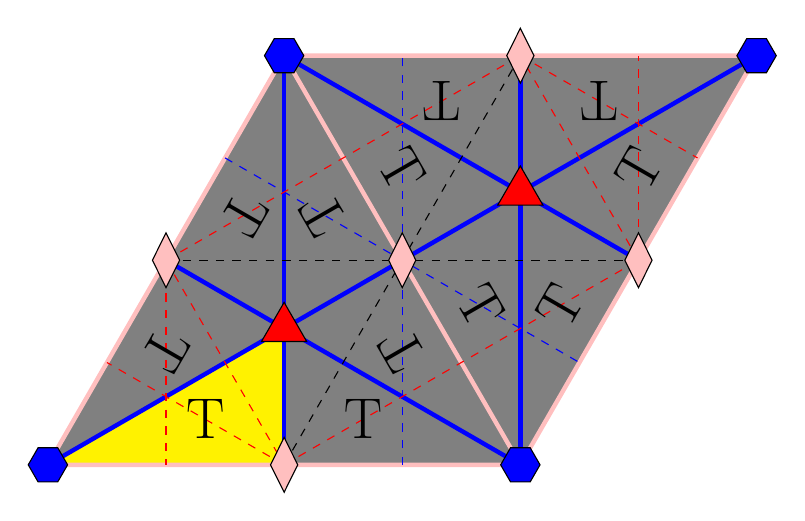
\begin{tikzpicture}
    % Define the lengths of the sides and the angle
    \def\a{3}  % length of side a
    \def\b{3}  % length of side b
    \def\angle{60}  % angle between sides a and b
    \def\s{T} % Label in center of cells

    % Calculate the coordinates of the points
    \coordinate (C00) at (0, 0);
    \coordinate (C10) at (\a, 0);
    \coordinate (C11) at ({\a + \b*cos(\angle)}, {\b * sin(\angle)});
    \coordinate (C01) at ({\b * cos(\angle)}, {\b * sin(\angle)});
    \coordinate (C02) at ({2*\b*cos(\angle)}, {2*\b * sin(\angle)});
    \coordinate (C12) at ({\a +2*\b * cos(\angle)}, {2*\b * sin(\angle)});
    \coordinate (C22) at ({2*\a + 2*\b * cos(\angle)}, {2*\b * sin(\angle)});
    \coordinate (C21) at ({2*\a + \b*cos(\angle)}, {\b * sin(\angle)});
    \coordinate (C20) at ({2*\a}, 0);

    \coordinate (A1) at ($(C00)!0.6666!(C11)$);
    \coordinate (A2) at ($(C11)!0.3333!(C22)$);

    % Draw the oblique unit cell
    \draw[fill=gray] (C00) -- (C20) -- (C22) -- (C02) -- cycle;
    \draw[thick,fill=yellow] (C00) -- (C10) -- ($(C00)!0.6666!(C11)$) -- cycle;
    \draw[ultra thick,pink] (C00) -- (C20) -- (C22) -- (C02) -- cycle;
    \draw[ultra thick,pink] (C20) -- (C02);
    \draw[ultra thick,blue] (C00) -- (C22);
    \draw[ultra thick,blue] (C01) -- (C20);
    \draw[ultra thick,blue] (C10) -- (C02);
    \draw[ultra thick,blue] (C02) -- (C21);
    \draw[ultra thick,blue] (C20) -- (C12);
    
    % Draw mirrow lines
    \draw[dashed,blue] ($(C01)!0.5!(C02)$) -- ($(C20)!0.5!(C21)$);
    \draw[dashed,blue] ($(C10)!0.5!(C20)$) -- ($(C02)!0.5!(C12)$);
    \draw[dashed] (C01) -- (C21);
    \draw[dashed] (C10) -- (C12);
    \draw[dashed,red] (C01) -- (C12);
    \draw[dashed,red] (C10) -- (C21);
    \draw[dashed,red] (C01) -- (C10);
    \draw[dashed,red] (C21) -- (C12);
    \draw[dashed,red] (C01) -- ($(C00)!0.5!(C10)$);
    \draw[dashed,red] (C10) -- ($(C00)!0.5!(C01)$);
    \draw[dashed,red] (C21) -- ($(C12)!0.5!(C22)$);
    \draw[dashed,red] (C12) -- ($(C21)!0.5!(C22)$);
    
    % Draw chiral center
    \node at ($(C00)!0.5!(C10)!0.3333!(A1)$) {\huge \s};
    \node[rotate=240] at ($(C00)!0.5!(A1)!0.3333!(C01)$) {\reflectbox{\huge\s}};
    \node[rotate=0] at ($(C10)!0.5!(A1)!0.3333!(C20)$) {\reflectbox{\huge \s}};
    \node[rotate=120] at ($(A1)!0.5!(C11)!0.3333!(C20)$) {\huge \s};
    \node[rotate=300] at ($(C11)!0.5!(A2)!0.3333!(C20)$) {\reflectbox{\huge \s}};
    \node[rotate=60] at ($(C21)!0.5!(A2)!0.3333!(C20)$) {\huge \s};
    \node[rotate=60] at ($(C21)!0.5!(A2)!0.3333!(C22)$) {\reflectbox{\huge \s}};
    \node[rotate=180] at ($(C12)!0.5!(A2)!0.3333!(C22)$) {\huge \s};
    \node[rotate=300] at ($(C11)!0.5!(A2)!0.3333!(C02)$) {\huge \s};
    \node[rotate=180] at ($(C12)!0.5!(A2)!0.3333!(C02)$) {\reflectbox{\huge \s}};
    \node[rotate=240] at ($(C01)!0.5!(A1)!0.3333!(C02)$) {\huge \s};
    \node[rotate=120] at ($(C11)!0.5!(A1)!0.3333!(C02)$) {\reflectbox{\huge \s}};

    % Draw node reflections
    \draw (C00)  node[regular polygon, regular polygon sides=6, draw, fill=blue, minimum size=0.5cm] {};
    \draw (C10)  node[shape aspect=0.5, diamond,draw,fill=pink] {};
    \draw (C11)  node[shape aspect=0.5,diamond,draw,fill=pink] {};
    \draw (C01)  node[shape aspect=0.5,diamond,draw,fill=pink] {};
    \draw (C02)  node[regular polygon, regular polygon sides=6, draw, fill=blue, minimum size=0.5cm] {};
    \draw (C12)  node[shape aspect=0.5,diamond,draw,fill=pink] {};
    \draw (C22)  node[regular polygon, regular polygon sides=6, draw, fill=blue, minimum size=0.5cm] {};
    \draw (C21)  node[shape aspect=0.5,diamond,draw,fill=pink] {};
    \draw (C20)  node[regular polygon, regular polygon sides=6, draw, fill=blue, minimum size=0.5cm] {};

    \draw (A1)  node[regular polygon, regular polygon sides=3, draw, fill=red, minimum size=0.5cm] {};
    \draw (A2)  node[regular polygon, regular polygon sides=3, draw, fill=red, minimum size=0.5cm] {};
\end{tikzpicture}
\end{document}